\subsection{Detektion mit MTCNN}
\begin{frame}
Verarbeitung von Multi-task Cascaded Convolutional Networks (MTCNN)
\begin{columns}
	\begin{column}{0.59\linewidth}<1->
\begin{itemize}
	\item<1-> Bildpyramide auf der Eingabe
	\item<1-> Die 3 Stufen:
	\begin{enumerate}
		\item<1-> Proposal Network (P-Net):
		\item<1-> Refine Network (R-Net):
		\item<1-> Output Network (O-Net):
	\end{enumerate}
	\item<1-> Non-maximum suppression (NMS)
	\item<1-> Zuverlässige Detektion und Erkennen von $20\times 20$ Pixel große Gesichter möglich.
\end{itemize}
	\end{column}
	\begin{column}{0.41\linewidth}<1->
		\centering
		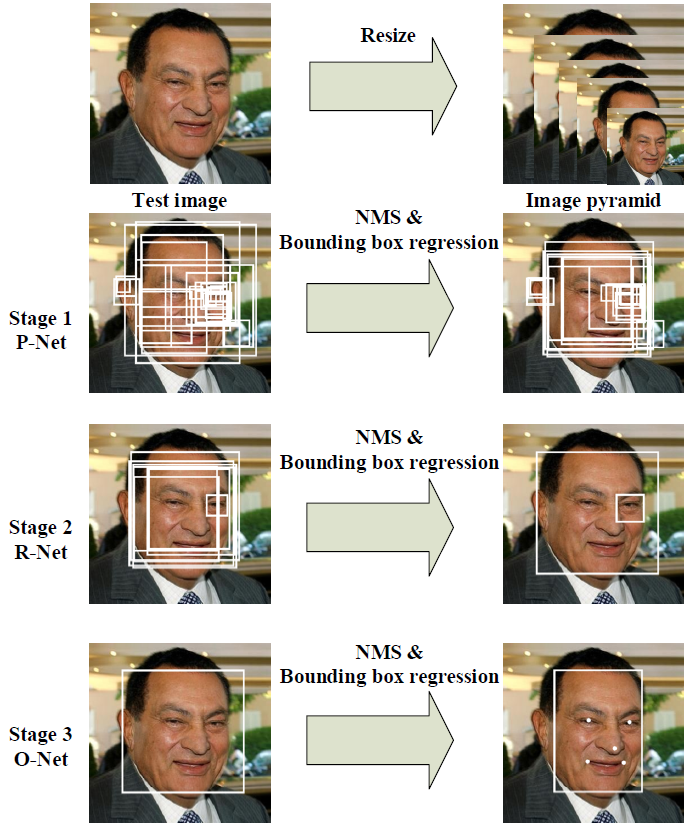
\includegraphics[width=\linewidth]{images/MTCNN_Step}
	\end{column}
\end{columns}
\end{frame}
\subsection{Verwendbarkeit im Versuch}
\begin{frame}
\begin{center}
	\begin{tabular}{|c|c|c|c|c|c|c|c|c|c|c|}
		\hline
		\tabbild[width=0.05\linewidth]{img_MTCNN/Img1-4_pupil1}&
		\tabbild[width=0.05\linewidth]{img_MTCNN/Img2-4_pupil1}&
		\tabbild[width=0.05\linewidth]{img_MTCNN/Img3-4_pupil1}&
		\tabbild[width=0.05\linewidth]{img_MTCNN/Img4-4_pupil1}&
		\tabbild[width=0.05\linewidth]{img_MTCNN/Img5-4_pupil1}&
		\tabbild[width=0.05\linewidth]{img_MTCNN/Img6-4_pupil1}&
		\tabbild[width=0.05\linewidth]{img_MTCNN/Img7-4_pupil1}&
		\tabbild[width=0.05\linewidth]{img_MTCNN/Img8-4_pupil1}&
		\tabbild[width=0.05\linewidth]{img_MTCNN/Img9-4_pupil1}&
		\tabbild[width=0.05\linewidth]{img_MTCNN/Img10-4_pupil1}&
		\tabbild[width=0.05\linewidth]{img_MTCNN/Img11-4_pupil1}\\
		{\fontsize{5}{7}$170\times235$}&
		{\fontsize{5}{7}$86\times118$}&
		{\fontsize{5}{7}$62\times87$}&
		{\fontsize{5}{7}$48\times65$}&
		{\fontsize{5}{7}$38\times54$}&
		{\fontsize{5}{7}$32\times44$}&
		{\fontsize{5}{7}$27\times39$}&
		{\fontsize{5}{7}$23\times31$}&
		{\fontsize{5}{7}$20\times26$}&
		{\fontsize{5}{7}$18\times24$}&
		{\fontsize{5}{7}$16\times21$}\\\hline
		$1m$& $2m$& $3m$& $4m$& $5m$& $6m$& $7m$& $8m$& $9m$& $10m$& $11m$\\\hline
	\end{tabular}
	Aufnahmen mit der Actioncam $(2688\times 1520, 170^\circ)$
\end{center}
\begin{itemize}
\item<1-> Detektion von Gesichtern bis zu $11m$ möglich
\item<1-> Ungenaue Landmarks für Augen, Nase und Mundwinkel
\end{itemize}
\end{frame}
